



\begin{figure}
    \centering
    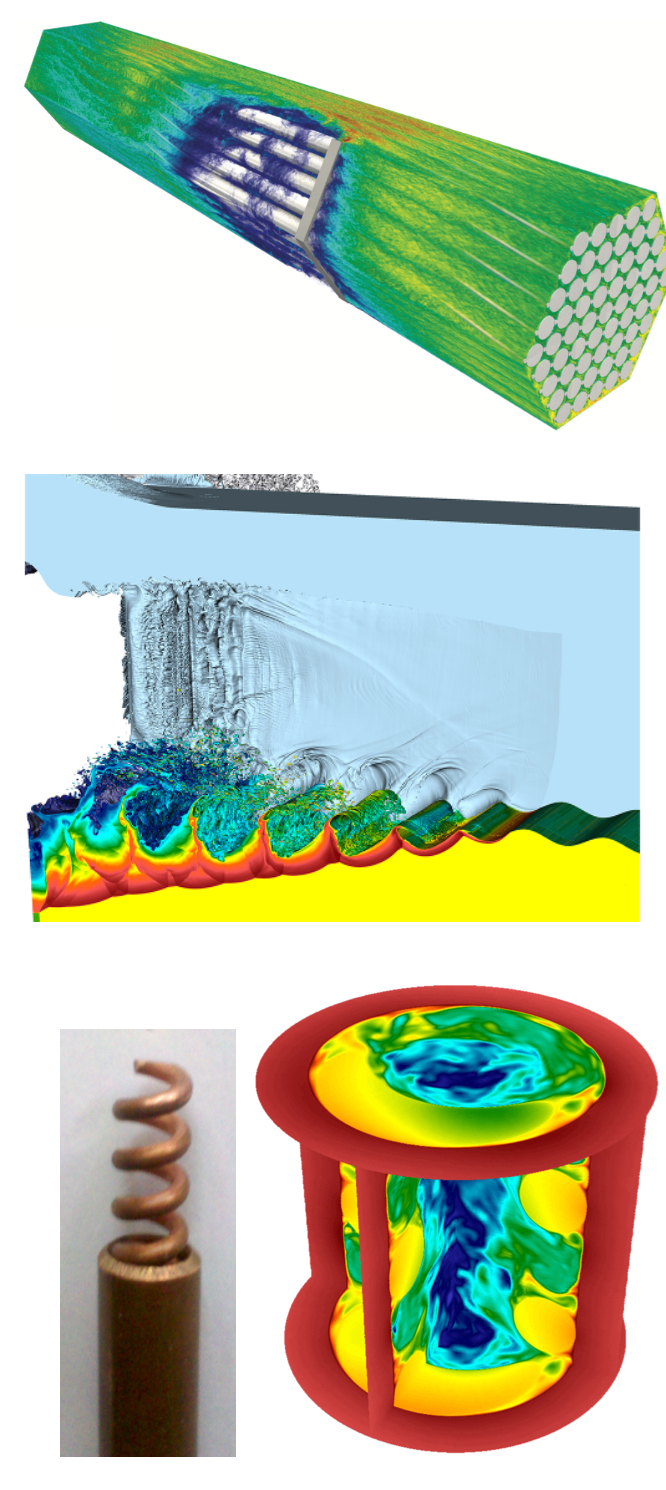
\includegraphics[width=0.15\linewidth]{../figs/collins1a_ppt.png}
    \hspace{.1in}
    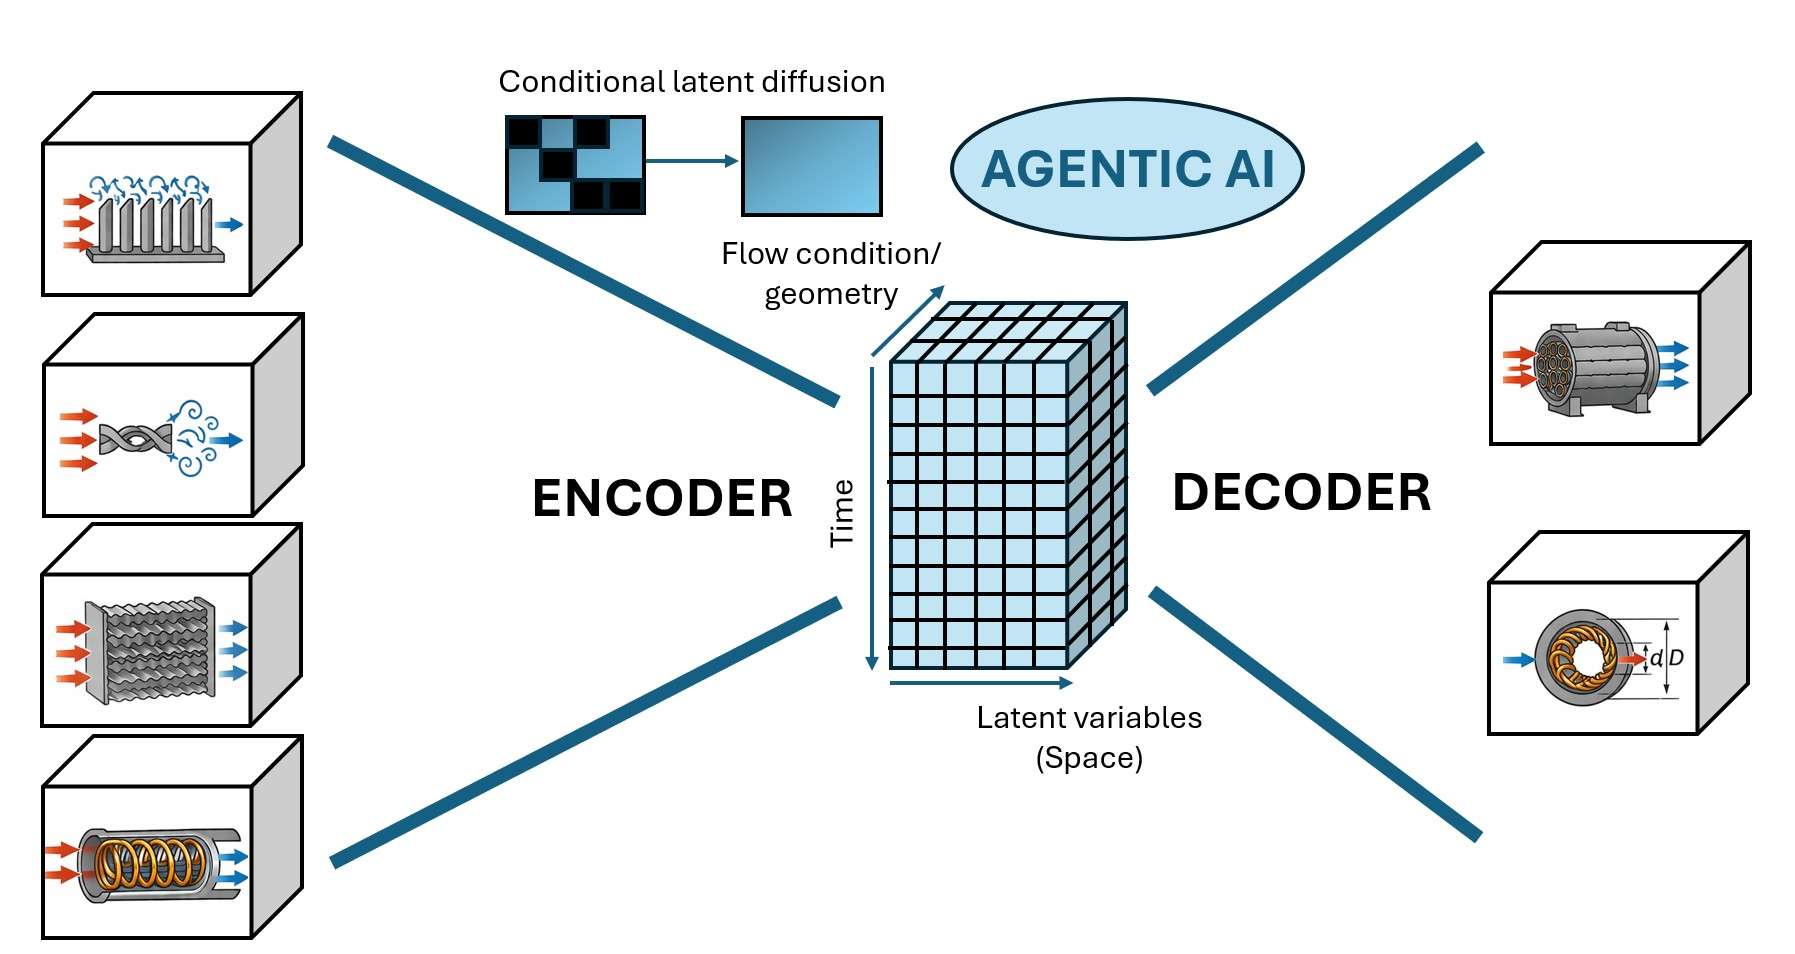
\includegraphics[width=0.70\linewidth]{../figs/fig_fm.jpg}
    \caption{Schematic representation of the proposed method combining a
foundation model with agentic AI. A wide range of high-quality fluid-flow
datasets are used to train a foundation model, which encodes all the cases into
a common latent space. Conditional latent diffusion is used to learn the
distribution across cases in the latent space. Spatio-temporal data for a new
geometry can be quickly produced in the latent space, and decoded back to the
physical space. The agentic AI framework has access to this foundation model
and the various optimizers, orchestrating the optimization/design process,
which is significantly accelerated.
{\bf WE WILL ADD TEST CASE IMAGES HERE, EITHER INTEGRATED OR STAND-ALONE}
} \label{fig:fm1}
\end{figure}

\section{Background/Introduction  -   1 PAGE}

{\color{gray} This project will develop a {\bf foundation-model–driven, agentic 
AI framework}~\cite{Vinuesa2026XAI} for the prediction, optimization, and 
control of thermal–fluid transport in energy systems, with primary emphasis 
on wire-wrapped fuel-rod bundles for advanced reactor design. These systems 
are central to DOE missions in advanced fission and fusion energy and are 
characterized by complex turbulent flows, strong geometric sensitivity, and 
stringent performance and safety requirements. They also constitute an 
exceptionally rich data domain, combining decades of high-fidelity simulations 
using Nek5000/RS--one of the few CFD codes accepted in NRC licensing workflows--with 
extensive experimental datasets from both open literature and proprietary industry sources.
The central objective of this {\bf Phase I effort} is to unify these 
heterogeneous datasets into a common representation and demonstrate a 
{\bf closed-loop workflow for rapid design and optimization}.
}

This project will develop a foundation-model-driven, agentic-AI
framework~\cite{Vinuesa2026XAI} for the prediction, optimization, and control
of thermal-fluid transport in energy systems, with primary emphasis on fission
and fusion applications.  These fluid systems represent a cornerstone of DOE’s
advanced energy programs and are characterized by complex turbulent flow,
strong geometry dependence, and stringent performance and safety constraints.
They also constitute a uniquely rich data domain, combining decades of
high-fidelity simulations using Nek5000/RS (one of the few CFD codes accepted
in NRC licensing workflows) and MFEM (the 2025 Gordon Bell Winner) with
extensive experimental datasets from both open literature and proprietary
industry sources. The central objective of this Phase I effort is to unify
these heterogeneous datasets into a common representation and demonstrate a
closed-loop workflow for rapid design and optimization.

Thermal-fluid transport is central to the majority of the world's energy
systems.  Nuclear reactors and fusion systems rely on fluid flow to transport
thermal energy from the core processes (fission/fusion reactions) to heat
exchangers, where working fluids are heated to drive turbines or other devices.
Combustion systems and inertially-confined fusion (ICF) systems rely on
repeatable fluid motion to initiate energy producting reactions.  System- and
device-level optimization, often involving domain-topology modifications, can
require hundreds of simulations, each of which can take days to months on
high-performance computing (HPC) platforms, depending on the domain complexity,
the range of timescales (e.g., convective-flow scales versus thermal-diffusive
scales in solids), and required fidelity.   

The overall goal of this project, to be realized in Phase II, is to radically
tranform the design cycle of energy system components by providing reliable and
accurate AI-driven surrogates coupled with state-of-the-art design optimization
[Sven?].  The targeted Phase I test problems are directly relevant to systems
in the DOE energy portfolio, including reactor cores and inertially confined
fusion (ICF).  (Liquid metal MHD for magnetically confined fusion will be
addressed in Phase II.) As illustrated in Fig. \ref{fig:fm1}, test cases for
Phase I include optimization of pressure-drop/heat-transfer in wire-wrapped
fuel-rod bundles, a miniapp for ICF, and optimization of wire-coil inserts for
heat transfer enhancement in beam-line devices.   These test cases were
selected because of the availability of reliable simulation and experimental
data and the fact that they can be scaled over a range of sizes, with the
number of simulation degrees-of-freedom (DOFs) ranging from $\sim 10^7$ to
$10^{12}$ \cite{gb23,gb25mfem}.

\section{    Project Objectives \hspace{1.0in} 1/2 PAGE}

\tiny \small \begin{verbatim}
   Provide a clear and concise statement of the specific objectives of the
   proposed project. Address how the objectives align with the chosen focus 
   topic and lead to an AI advantage.

      Misun / Elia / Dillon
\end{verbatim} 
\normalsize



\vspace*{1in}
\section{    Proposed Research and Methods \hspace{1.0in} 1-1/2 PAGES}

\tiny \begin{verbatim}
  Provide a clear research plan for a 9-month project and describe the proposed activities and methods. 

  Include enough technical details to evaluate the impact of the proposed activity. 

  For each activity, indicate the responsibility of the key investigator(s) and the associated budget.  
  If the proposed application is building on an existing, currently funded DOE project, describe how 
  the submitted application leverages that work and is distinct from the existing funding.

  Here building on Vlad and Ricardo's text; ANYONE - please jump in 
\end{verbatim} 
\normalsize

{\color{gray}
The first component of the research plan focuses on the development of a {\bf geometry-aware 
thermal–fluid foundation model}, led by ANL, UIUC, and PSU. Building on prior work in foundation 
modeling~\cite{Vishwasrao2026AgenticPDE}, simulation and experimental data from 
wire-wrapped bundles~\cite{Dai2025WireWrapped61Pin,kaeri37pin}, as well as related configurations 
such as spacer grids, pebble beds, and twisted tubes, will be mapped into {\bf a common latent 
space independent of mesh topology}. This capability is particularly critical for reactor applications, 
where variations in geometry—such as wire pitch, rod spacing, and bundle configuration—strongly 
influence heat transfer and pressure losses.
The proposed model integrates {\bf graph-based geometric representations}, 
{\bf variational autoencoders (VAEs)} for compression of high-dimensional flow 
fields~\cite{Vinuesa2022MLCFD,SoleraRico2024BetaVAE},
and {\bf conditional latent diffusion models}~\cite{Vishwasrao2025DiffSPORT} 
to learn distributions across operating regimes. 
Training will leverage DOE exascale-ready workflows and GPU-enabled datasets generated using 
{\bf Nek5000/RS} and {\bf MFEM}. The resulting surrogate model will enable fast, high-fidelity 
prediction of key reactor performance quantities, including heat transfer coefficients, 
pressure drop, and flow-induced mixing. For the cases considered, we have already established
clear agreement between the experimental data and the high-order simulation codes, which will be 
used to validate the ML surrogates.

The second component develops a {\bf latent-space optimization and control framework}, 
led by the University of Michigan, targeting both steady and transient operating regimes. 
This effort will employ a hybrid strategy combining {\bf Bayesian optimization}~\cite{Morita2022BOCFD}, 
{\bf derivative-free optimization methods}, and {\bf reinforcement learning}~\cite{Font2025DRLFlowControl. 
Such approaches are essential for reactor-relevant design spaces that are high-dimensional, 
non-convex, and constrained by safety and operational limits.

Optimization will be performed directly within the latent space of the foundation model, 
enabling efficient exploration of design variables such as wire pitch, rod arrangement, 
and operating conditions. The {bf agentic AI system} will orchestrate this process by dynamically 
selecting optimization strategies, proposing new simulation queries, and balancing competing 
objectives, including heat transfer enhancement, pressure loss minimization, and 
safety margin preservation.
}

\medskip
The first component of the research plan focuses on the development of a
geometry-aware foundation model for thermal-fluid prediction, led by ANL,
UIUC, and PSU.  
Building on prior work on foundation models~\cite{Vishwasrao2026AgenticPDE}, as
well as simulation and experimental data from wire-wrapped bundles
\cite{Dai2025WireWrapped61Pin,kaeri37pin}, and related configurations such as
spacer grids, pebble beds, and twisted tubes, results will be mapped to a
common latent space independent of mesh topology.
%
This is particularly critical for reactor applications, where geometry
variations (wire pitch, rod spacing, bundle configuration) strongly influence
heat transfer and pressure losses. 
  The model will combine graph-basedrepresentations of geometry, variational
autoencoders for compressing high-dimensional flow
fields~\cite{Vinuesa2022MLCFD,SoleraRico2024BetaVAE}, and conditional latent
diffusion~\cite{Vishwasrao2025DiffSPORT} to learn the latent distribution
across operating regimes. 
%
Training will exploit available experimental data sets (e.g.,
\cite{kaeri37pin}) and DOE exascale-ready workflows and GPU-enabled
datasets from Nek5000/RS The resulting surrogate will provide fast, accurate
predictions of quantities central to reactor design and licensing, including
heat transfer coefficients, pressure drop, and flow-induced mixing.
   For the cases considered, we have already established clear agreement
between the experimental data and the high-order simulation codes, which
will be used to validate the ML surrogates.

The second component develops a latent-space optimization and control
framework, led by the University of Michigan, targeting both steady and
transient regimes. We will employ a hybrid strategy combining Bayesian
optimization~\cite{Morita2022BOCFD}, derivative-free methods, and reinforcement
learning~\cite{Font2025DRLFlowControl}. This is essential for reactor-relevant
design spaces, which are high-dimensional, non-convex, and constrained by
safety and operational limits. Optimization will be performed directly in the
latent space of the foundation model, enabling efficient exploration of design
parameters such as wire pitch, rod arrangement, and operating conditions. The
agentic-AI system will orchestrate this process by selecting optimization
strategies, proposing new simulation queries, and balancing competing
objectives such as heat transfer enhancement, pressure loss, and safety
margins. The framework will operate in a closed loop, where candidate designs
generated in latent space are selectively validated using high-fidelity
simulations, ensuring both accuracy and robustness.

The third component focuses on validation across multiple DOE-relevant
applications and integration into the Genesis Mission ecosystem, led by Argonne
with contributions from all partners. In addition to wire-wrapped reactor
bundles, we will consider two complementary applications that expand the scope
and generality of the approach. The first is inertial confinement fusion, where
highly transient, multiphysics dynamics arise from laser-driven compression of
fuel pellets. This provides a stringent test of the model’s ability to capture
fast-evolving regimes. The second is a well-characterized heat transfer
enhancement problem involving wire-coil inserts in cooling channels, where
experimental data \cite{collins22}) show up to fourfold increases in heat
transfer with well-quantified pressure penalties. 
%
   This problem is particularly valuable for model development and validation
due to the sensitivity of the QOI (typically the Nusselt number), its rich
parameter space (wire diameter, pitch, Reynolds number), strong agreement
between simulations and experiments, and relatively low cost for simulation data.

The MFEM team will contribute a targeted ICF miniapp designed primarily as a
high-fidelity data generator for training and validating the proposed surrogate
modeling framework. Building on existing capabilities in Lagrangian
hydrodynamics \cite{Dobrev2012}, ALE methods \cite{Tomov2018}, and scalable
H(div) radiation diffusion solvers \cite{Pazner2025}, this effort will focus on
producing physically consistent, multi-physics datasets that capture coupled
hydrodynamics–radiation behavior across parameterized geometries and operating
conditions. The miniapp will be tightly integrated into the AI workflow to
systematically generate training data, support active learning loops, and
enable evaluation of surrogate accuracy and generalization. In Phase I,
simplified ICF configurations will be used to demonstrate feasibility and
establish a robust pipeline connecting MFEM-generated data with the foundation
models, ensuring that learned representations remain consistent with the
underlying physical operators and constraints.

This effort directly complements the proposed AI architecture by providing
high-order, structure- preserving finite element data that aligns with the
project’s emphasis on physically consistent latent spaces. MFEM’s support for
complex, unstructured meshes and high-order discretizations enables systematic
variation of geometry and resolution, which is critical for training
geometry-aware models such as GNN-based encoders. Moreover, the compatibility
of MFEM operators with differentiable programming frameworks enables a natural
pathway to incorporate operator-level sensitivities into both surrogate
training and downstream optimization. This creates a strong link between the
simulation stack and the latent-space optimization strategies outlined in the
proposal, particularly for adjoint-informed refinement and hybrid optimization
workflows.

  Together, these Phase I applications provide relatively wide coverage of 
energy-relevant thermal-fluids systems.
This effort builds directly on DOE investments in high-fidelity simulation.
Nek5000/RS and MFEM are Gordon Bell Prize winning codes
\cite{tufo99a,gb23,gb25mfem} developed under the Center for Efficient Exascale
Discretizations as part of DOE's Exascale Computing Project.  Their high-order
discretizations, coupled with fast matrix-free operator evaluation and highly
scalable preconditioners gives them a competitive edge over traditional approaches
(e.g., a 32X gain compared to 2nd-order finite volumes for $Re=50$M
boundary-layer flows \cite{Min2024Wind,Tomboulides2024ABL}).  Nek5000/RS has
been extensively used for reactor thermal-hydraulics and is part of
NRC-accepted workflows. The proposed work, however, is fundamentally distinct.
Instead of advancing simulation capabilities alone, we develop a generalizable
foundation model that unifies data across geometries and regimes, and we
introduce a closed-loop, AI-driven optimization framework that enables rapid
design exploration and mechanistic discovery. By the end of Phase I, we will
demonstrate real-time surrogate modeling and closed-loop optimization for
representative thermal-fluid systems, establishing a clear pathway toward
AI-driven digital twins for reactor design and other DOE mission applications.


\vspace*{.1in}
\noindent {\bf Effort Breakdown:}
   {\bf ANL}-reactor TF data; model validation; device optimization \$100K;
   {\bf LLNL}-ICF data; model validation \$100K;
   {\bf U. Mich.}-model development; device optimization \$100K;
   {\bf PSU}-reactor TF data; model validation \$50K;
   {\bf UIUC}-heat-exchanger data; model validation \$50K.


\newpage
\section{  Milestones in the Nine Months \hspace{1.0in} 1 PAGE}

\tiny \small \begin{verbatim}
  Misun, Ricardo, Luke
  Provide a list of clearly defined and measurable milestones of the project.
\end{verbatim} 
\normalsize

\newpage
\section{    Data Sources and Models \hspace{1.0in} 1/2 PAGE}

\tiny \begin{verbatim}
  Misun, Paul, Tzanio, Dillon  (pay attn to APPENDIX 2)

  Describe which existing or new data sources will be used. Address your team’s access to the data.  
  If applicable, indicate which AI models or frameworks will be used in your proposed project.  
  Do not include a computing resources--to be done in Appendix 2.

  Here, discuss: o  Experimental data for fuel pins \cite{KAIST,Todreas}
                 o  Nek5000/RS and MFEM as trusted high-accuracy and efficient sources
                 - Top-ranked in numerous benchmark cases (T-junction \cite{tjunc}, 5-pin spacer grid \cite{5pin}, etc.)
                 - 1/32 the amount of computational resources as FV for the same accuracy for Re=50M 
                   boundary layer calculation (1/8 the number of grid points, 1/2 the number of timesteps, 
                   and 1/2 the time per step, per gridpoint on the same platform, OLCF Summit)

 o  Collins data for the small wire-coil - both experimental and numerical results available 
\end{verbatim} 
\normalsize

\noindent
{\bf Dillon, Elia, I wonder if this is a reasonable place to put Experimental/Numerical Comparison
Results?  For example, as here:}
\begin{figure}[h] 
 \centering {\setlength{\unitlength}{1.00in}
   \begin{picture}(2.0,1.5)(0,0)
      \put(0.0,0.0){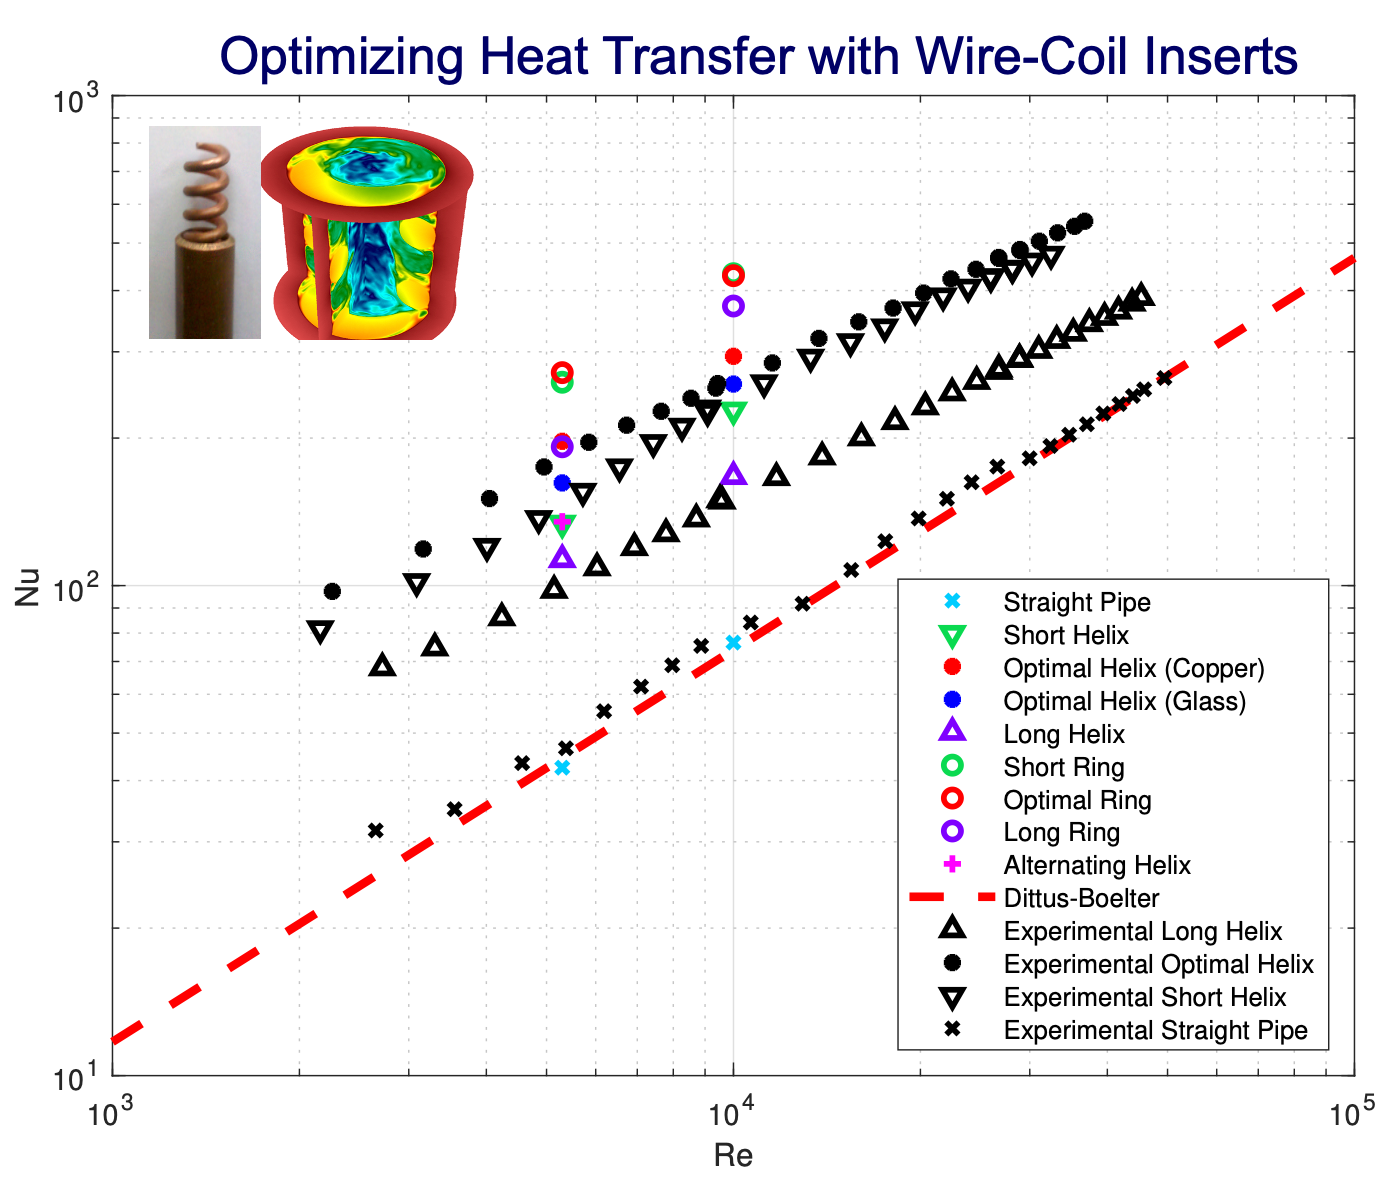
\includegraphics[height=1.5in]{../figs/collins_02_nek_nu3.png}}
   \end{picture}}
\caption{\label{fig:collins}
Experimental-Nek5000/RS data comparison of Nusselt number
vs. Reynolds number for various wire-coil insert geometries \cite{kaneko22}.
}
\end{figure}
\vspace*{.1in} 

%%%%%%%%%%%%%%%%%%%%%%%%%%%%%%%%%%%%%%%%%%%%%%%%%%%%%%%%%%%%%%%%%%%%%%%%%%
%\begin{wrapfigure}{r}{0.4\textwidth}
% \centering {\setlength{\unitlength}{1.00in}
% \begin{picture}(2.0,1.5)(0,0)
%     \put(0.0,0.0)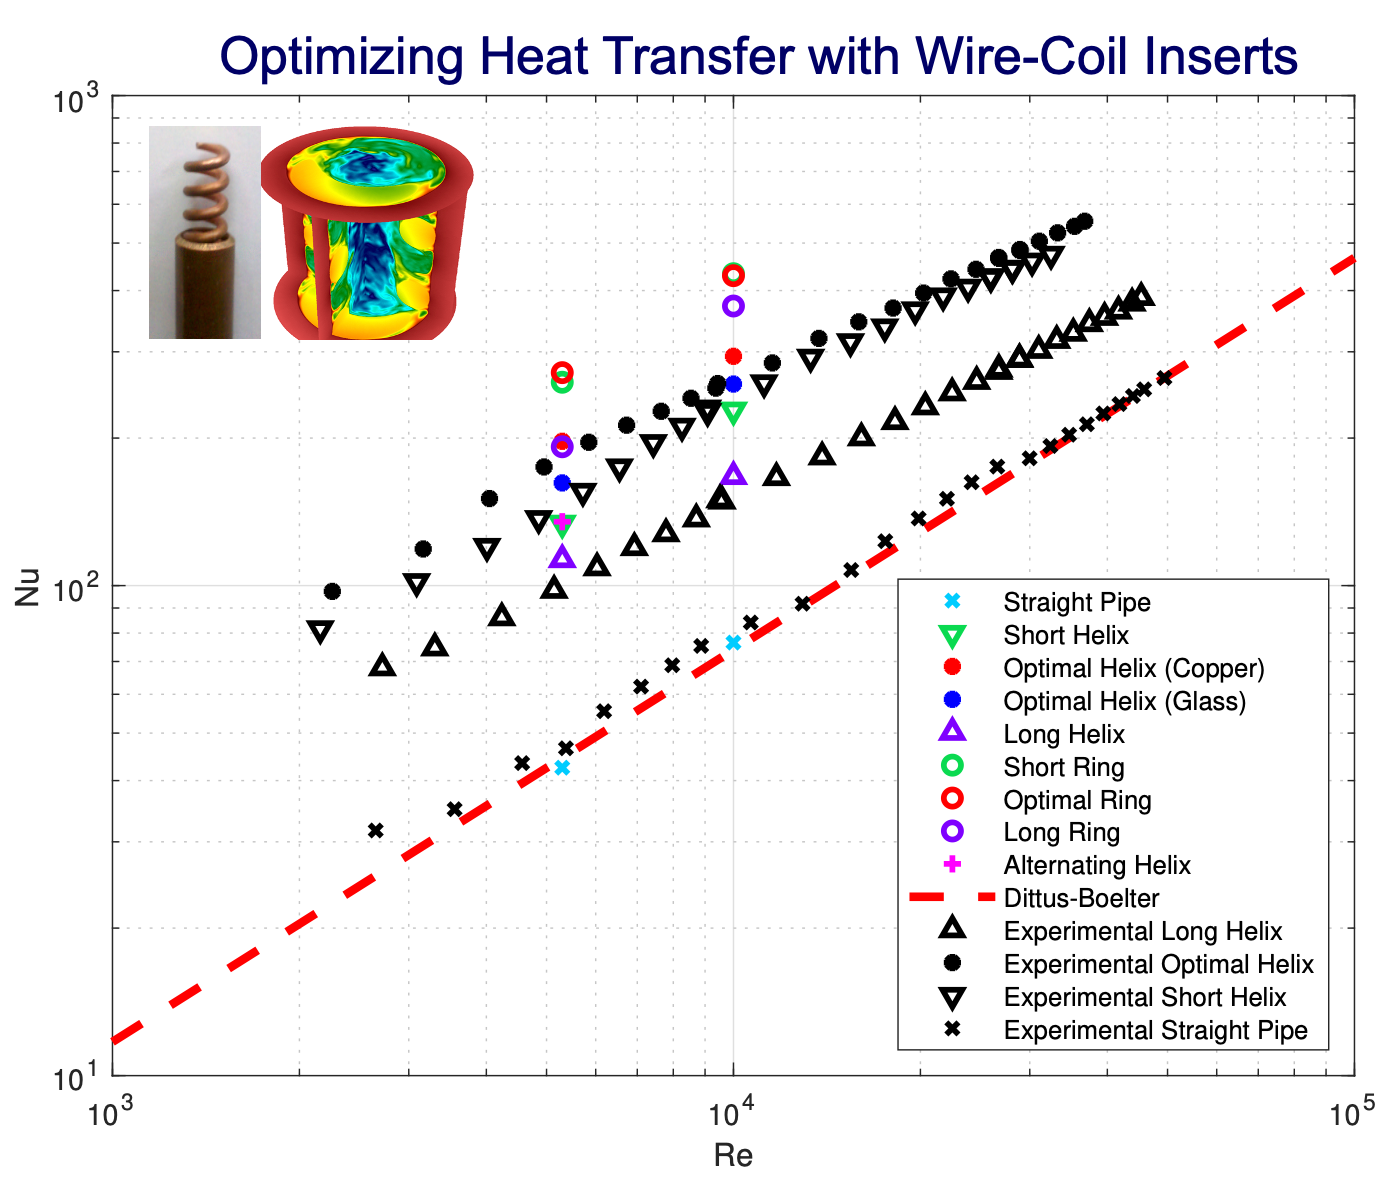
\includegraphics[width=0.4\textwidth]{../figs/collins_02_nek_nu3.png}
%    \end{picture}
%  }
%    \caption{\label{fig:collins}
%    Experimental-Nek5000/RS data comparison of Nusselt number
%    vs. Reynolds number for various wire-coil insert geometries \cite{kaneko22}.
%    }
% \end{wrapfigure}
%%%%%%%%%%%%%%%%%%%%%%%%%%%%%


{\bf These two pars. need work... They are sort of just filler for the moment. PFF.}
The Argonne team has extensive experience in large eddy simulation (LES) of
turbulent flow in reactor, including everything from isolated subassemblies
\cite{fischer08a,Dai2025WireWrapped61Pin,other} to full cores \cite{sc22,gb23,other3}.
The majority of these simulation datasets are still available and summarized in
the nuclear engineering literature.  Additional data can be readily generated
using Nek5000/RS on existing compute resources on OLCF Frontier, ALCF Aurora,
or the NE Divison cluster, {\em Nek5000}, as part of ongoing studies.  The
generation of wire-wrapped fuel bundle geometries has been fully automated so
that model training at new points in the the wire-wrap diameter / pitch space
is straightforward.  This validity of this simulation data is backed up through
extensive comparisons with experiments.  The latest (and most detailed) data
for wire-wrapped bundles is available in \cite{kaeri37pin}, which will also be
used for model training. {\bf Make a comment about the size/cost of the
simulations that we are contemplating.}

The data situation is similar for the wire-coil insert geometry, which is a
low-cost case to be used for test/development of the overall workflow.
Extensive high-quality data is available in \cite{collins22}, which has been
corroborated with Nek5000/RS studies by Kaneko, who also examined nearby
geometric configurations such as arrays of ring inserts \cite{kaneko22}.
These cases are sufficiently small that they can run on just one or two
GPUs for one hour to generate requisite heat-transfer QOIs (e.g., Nusselt
number, Nu, which is the nondimensional heat-transfer coefficient).
It is also a case where the QOI is sensitive to geometry, with up to a
4$\times$ increase in Nu observed in experiments and simulations for
the best configurations, implying that there is a clear optimization win
to be had in this case that should be found automatically by the proposed
AI framework.


\section{    Decision Gate Metrics \hspace{1.0in} 1/2 PAGE}

\tiny \small \begin{verbatim}
  Ricardo / Luke / Misun 

  Provide specific metrics that can be used for the evaluation of Phase I go/no
  go decision. 

  DOE encourages the development of metrics to identify AI advantage. 
  One such metric could include scaling behavior which shows increasing performance
  as additional data, computing, and/or other resources are applied. 

  Quantitative statements enabling transformative science and engineering through AI are preferred.
\end{verbatim} 

\normalsize


